\chapter{Analysis of Reliability}

\section{Test Objectives}

The test campaigns presented here aim to investigate the reliability of UDP communication in a local network under conditions similar to those in the distributed Test Support System. Reliability is measured by the number of lost packets. Both topologies presented in \ref{chap:Architectures} were considered.

Packet loss can occur at several points within the network. On the one hand, it can be caused by a participating computer system. Possible causes include an overflow of the socket receive buffer or the network interface buffer (RX\_Ring or TX\_Ring). The QDisc queue, which is used in the network stack to send packets, can also overflow. In addition, limited system resources, such as CPU and memory contention or high interrupt handling, can also lead to packet loss.

In the tests using the star topology with a switch in the centre (see \ref{chap:TopoSwitch}), packet loss may also occur due to this switch. Possible reasons for this are exceeding the maximum switch capacity, which is 160 GBit/s, or an egress buffer overflow. These buffers have a size of 6 MB, and are dynamically shared between all ports \cite{setup09}.

\section{Reliability Analysis of the Star Topology with a Switch in the Centre}

\subsection{System under Test}
The test campaigns presented in this chapter utilize the star topology with a switch in the center (see \ref{chap:TopoSwitch}). All systems are connected to each other through the Cisco CBS350-8XT switch. The network interfaces mentioned in the architecture presentation are utilized in the computer systems.

\begin{figure}[h!]
    \centering
    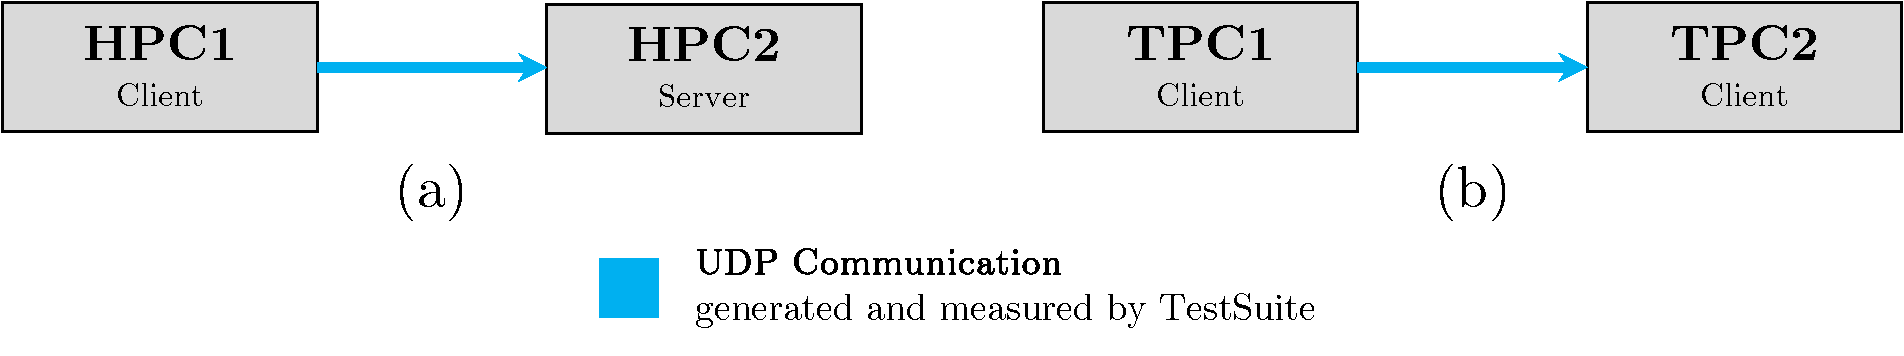
\includegraphics[width=1\linewidth]{figures/reliability/star/rel_g_1.pdf}
    \caption{Illustration of the used Systems under Test.}
    \label{fig:sutreliability}
\end{figure}

One system under test is a UDP communication generated by the Test Suite between the two High-Performance PCs (see Figure \ref{fig:sutreliability}a). HPC1, is the sender, also referred to as the client, and HPC2 is the receiver, also referred to as the server. Additionally, tests were conducted using the two Traffic PCs as the system under test (refer to Figure \ref{fig:sutreliability}b).

\subsection{Test Campaings}

\subsubsection{Isolated Tests in Different Operating States} \label{chap:relcamp1}
\paragraph{Motivation and Context}

As mentioned above, certain operating conditions can cause packet loss due to limited system resources. The purpose of this campaign is to identify the type of load on the test setup that causes packet loss. The following operating states are considered:

\begin{itemize}
  \item \textbf{System without any additional Load}
  \item \textbf{CPU Load} in User Space, Kernel Space and by Real-Time Processes (see \ref{chap:stressngCPU})
  \item \textbf{Memory Load} (see \ref{chap:stressngMemeory})
  \item \textbf{I/O Load} on internal Hard Disk (see \ref{chap:stressngIO})
  \item \textbf{Load due to Timer Interrupts} (see \ref{chap:stressngInterrupt})
  \item \textbf{Network Load} \\
  		Additional network load was generated with a participating computer system of the system under test. In the example of the High-Performance PCs as the SuT, this means UDP communication between the client or server and a Traffic PC. The Traffic PC is acting as the sender, and the respective computer system of the SuT is acting as the receiver.
  		
  \item \textbf{Traffic Load} \\
 		Traffic Load refers to bi-directional UDP communication between computer systems that are not part of the current system under test. The objective is to strain the switch.
\end{itemize}

The tools presented in \ref{chap:loadgeneration} are used to generate this load. The system is tested under maximum load. This means that as many stressors are used for the load generated with stress-ng as the system has logical CPU cores. A bandwidth of 10 GBit/s is used for the network stressors.

The presented operating states were tested individually for client and server. The two Traffic PCs as well as the High-Performance PCs were used as the system under test. The test duration for all tests was 100 seconds and a cycle time of 0 µs was used, whereby the maximum possible bandwidth was used for transmission. The datagram sizes used were 80 bytes as a representative for small datagrams in the test support system, 8900 bytes as a datagram size close to the MTU, and 65000 bytes as a datagram size close to the maximum of UDP.

\paragraph{Results}
In tests where the client was subjected to a generated load, no packet loss was detected in any of the tested operating states. This applies to both the tests with High-Performance PCs and Traffic PCs as a system under test.

\begin{figure}[h!]
  \centering
  \subcaptionbox{High-Performance PCs as System under Test\label{fig:resuc1a}}{%
    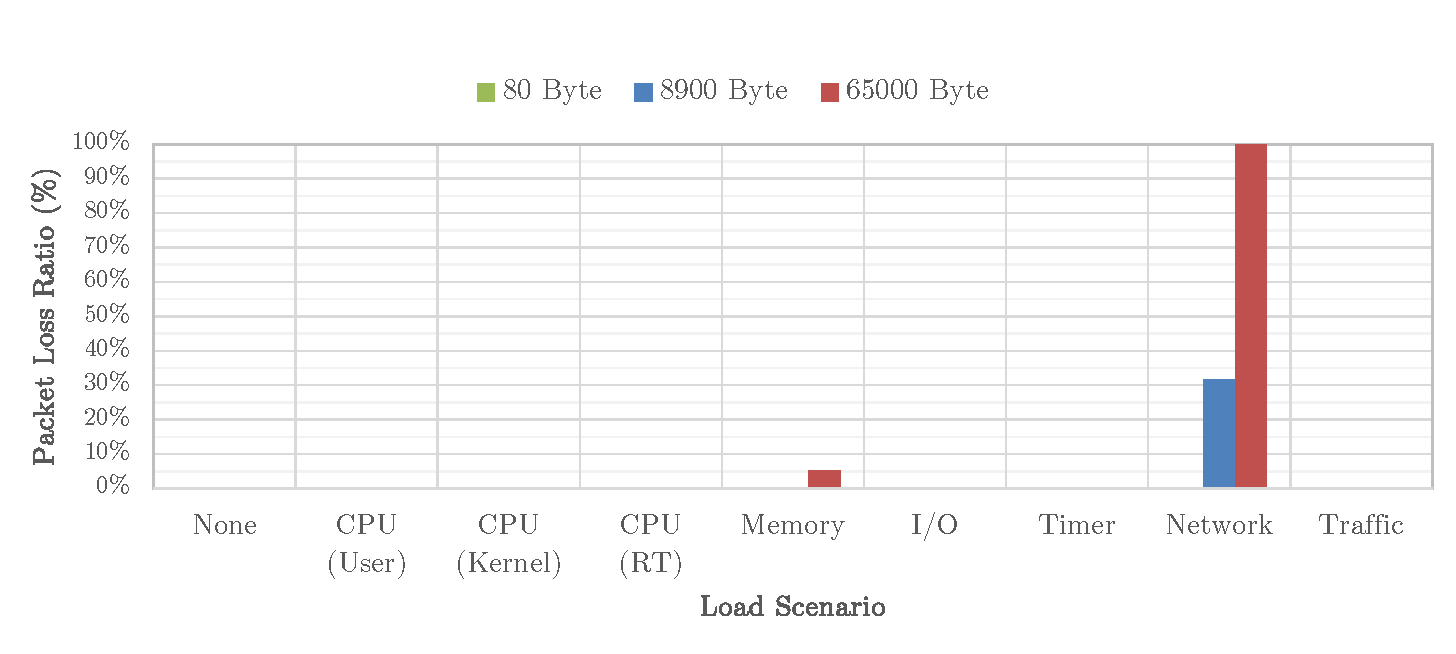
\includegraphics[width=1\textwidth]{figures/reliability/star/rel_d_1a.pdf}
  }
  \subcaptionbox{Traffic PCs as System under Test\label{fig:resuc1b}}{%
    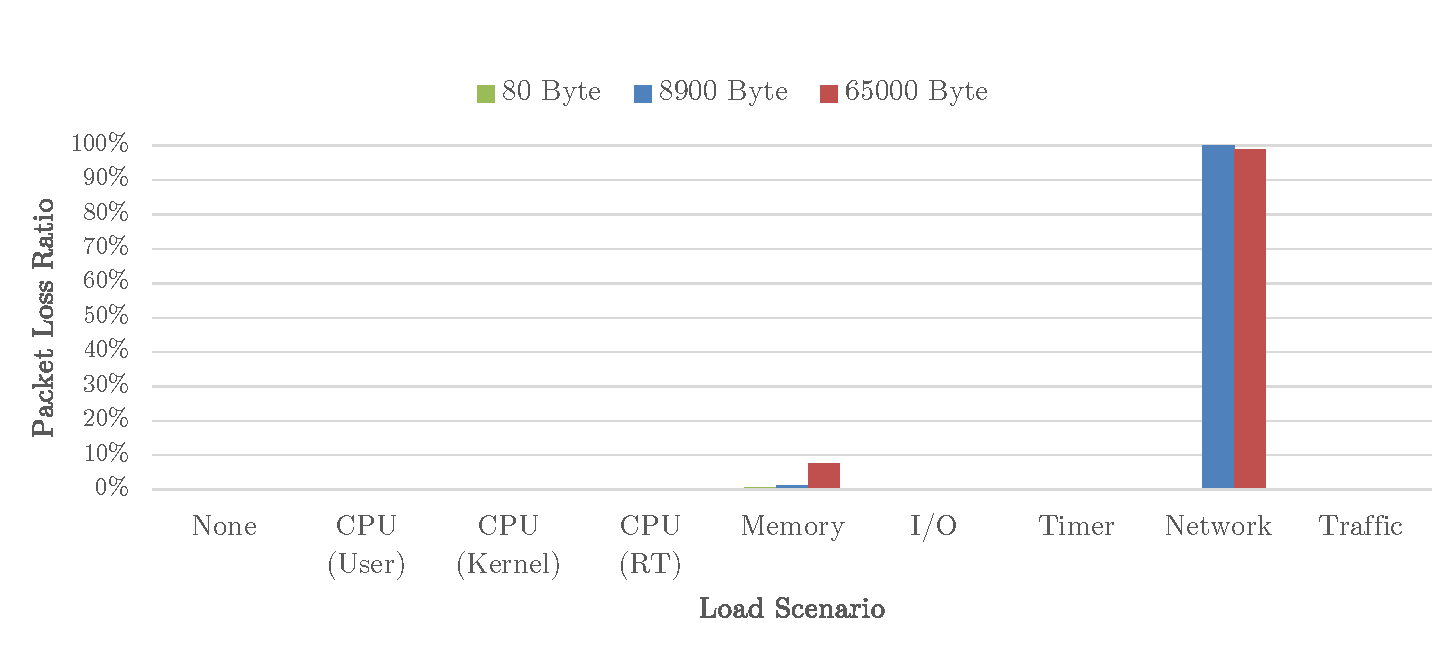
\includegraphics[width=1\textwidth]{figures/reliability/star/rel_d_1b.pdf}
  }
  \caption{Packet Loss Ratio for various Load Scenarios with different Datagram Sizes (Campaign 'Isolated Tests in Different Operating States').}
  \label{fig:resuc1}
\end{figure}

During the stress tests where the server was subjected to a generated load, packet losses occurred on both systems under test. Figure \ref{fig:resuc1a} displays the percentage of packet losses in different load scenarios for High-Performance PCs, while Figure \label{fig:resuc1b} shows the results for Traffic PCs. The diagrams demonstrate that packet losses occurred in both systems under test when subjected to the stress-ng 'bigheap' stressor which generates memory load and to network load on the server.

Under stress from memory load, the server experiences packet losses across all three datagram sizes tested. Losses are less than one percent for 80 and 8900 bytes, which is why they are not visible on the diagram. However, they increase to 5.29\% and 7.81\% for 65000 bytes, which is due to fragmentation, since the entire datagram is lost when a fragment is lost. It is also observed that the losses are slightly lower with the High-Performance PC as the system under test compared to the Traffic PC as the system under test when under memory load.

The losses occurred in the server, and the network card dropped the packets, as determined by the standard interface statistics of the network interface in the server. The drops occur due to memory load, as explained in \ref{chap:stressngMemeory}. This results in insufficient memory to process the arriving packets through the network stack. For instance, the network stack may not be able to allocate a socket buffer structure to process an incoming packet.

Additionally, packet losses have been observed with network load for datagram sizes of 8900 and 65000 bytes. These are due to the maximum bandwidth being exceeded because both the client and another computer system are sending data to the server at up to 10 Gbit/s. As a result, the maximum bandwidth of 10 GBit/s, with which the server is connected to the switch, is exceeded, which is why packets get dropped by the switch.

\begin{figure}[htbp]
  \centering
  \subcaptionbox{Datagram Size of 80 Byte\label{fig:resuc2a}}{%
    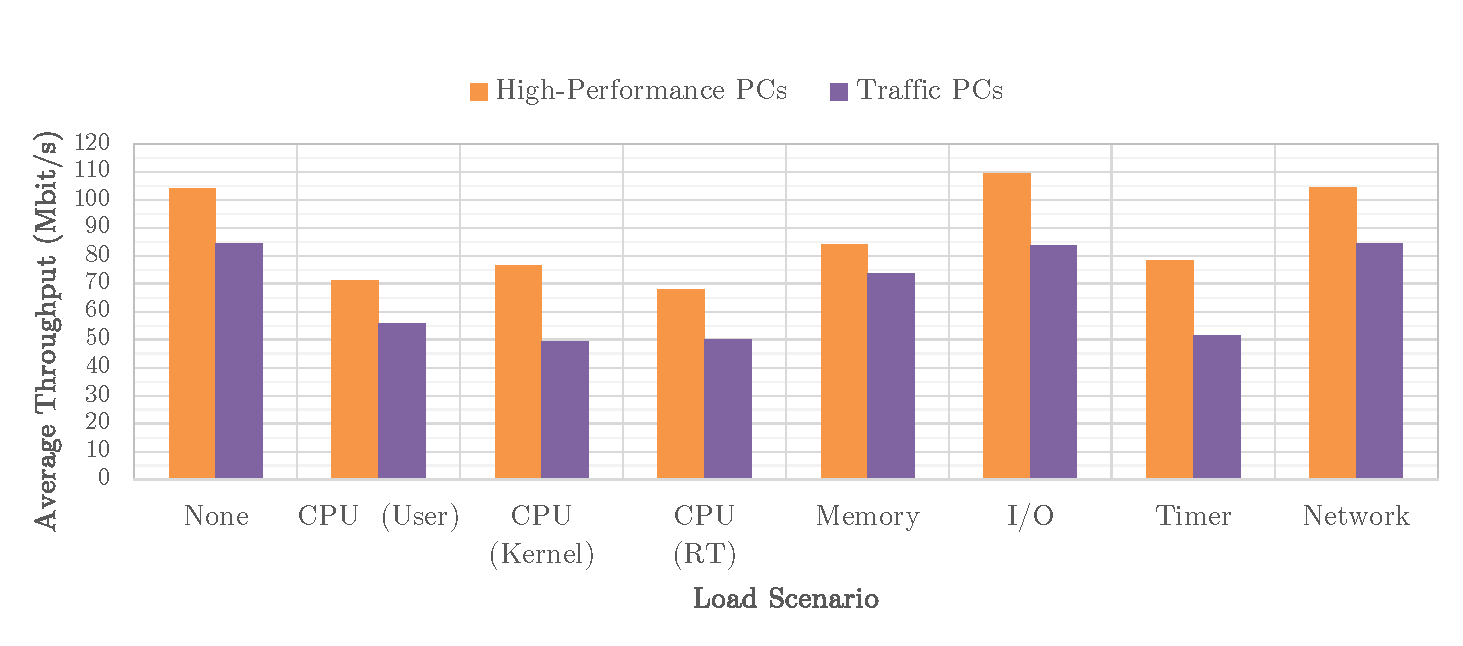
\includegraphics[width=0.9\textwidth]{figures/reliability/star/rel_d_2a.pdf}
  }
  \subcaptionbox{Datagram Size of 8900 Byte\label{fig:resuc2b}}{%
    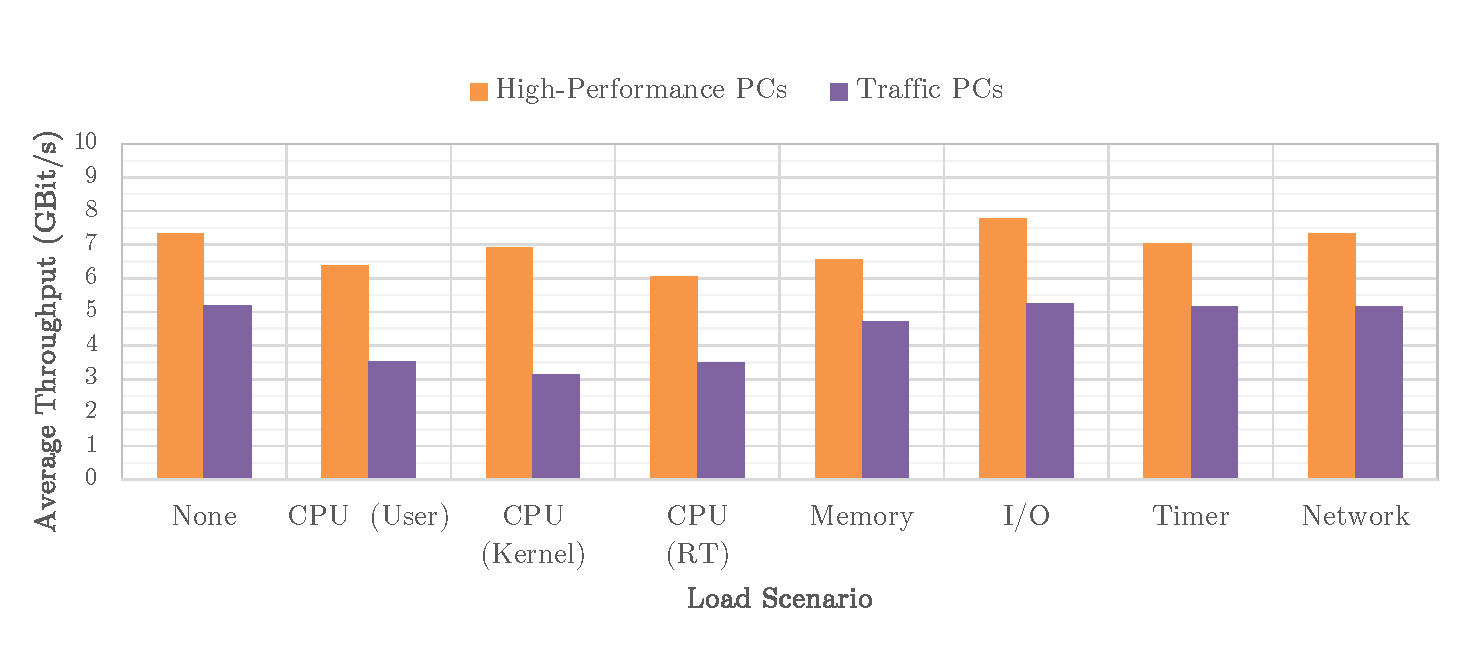
\includegraphics[width=0.9\textwidth]{figures/reliability/star/rel_d_2b.pdf}
  }
    \subcaptionbox{Datagram Size of 65000 Byte\label{fig:resuc2c}}{%
    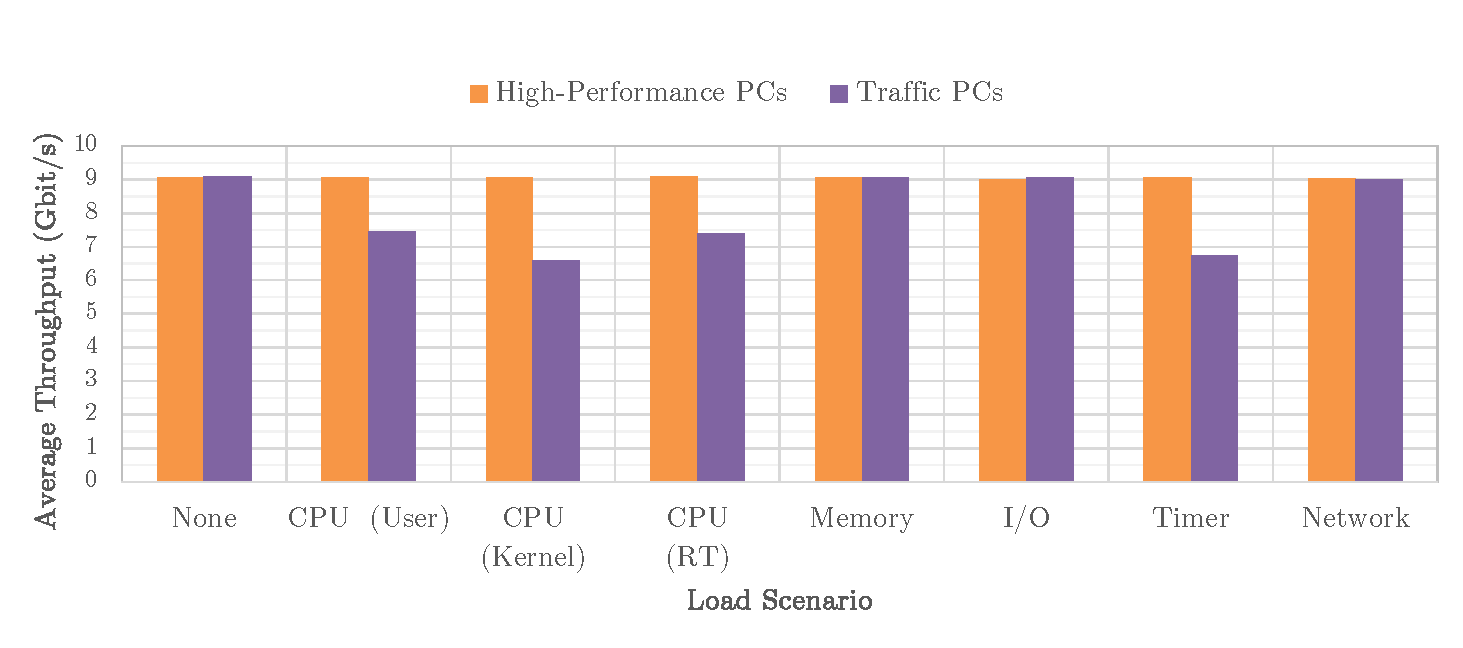
\includegraphics[width=0.9\textwidth]{figures/reliability/star/rel_d_2c.pdf}
  }
  \caption{Average Throughput for various Load Scenarios (Campaign 'Isolated Tests in Different Operating States').}
  \label{fig:resuc2}
\end{figure}

As mentioned above, there were no packet losses during the tests where the client was loaded. However, the stress did affect the average throughput sent to the server. Figure \ref{fig:resuc2} compares the average throughput of the High-Performance PCs and Traffic PCs as system under test in different operating conditions.

On one side, the average throughput of the High-Performance PCs is higher than that of the Traffic PCs, especially for datagram sizes of 80 bytes and 8900 bytes. All categories of CPU load, memory load, and load due to timer interrupts have a negative impact on the average throughput, with a reduction of 5\% to 10\% greater for Traffic PCs than for High-Performance PCs, particularly for datagram sizes of 80 bytes and 8900 bytes.  At 65,000 bytes, the throughput of High-Performance PCs remains unaffected by any stress, while the throughput of Traffic PCs is reduced by up to 25\% by CPU and timer interrupt load.

These differences in average throughput and the impact of additional system load on it are due to differences in hardware. The hardware of High-Performance PCs is significantly more powerful than that of Traffic PCs (see \ref{chap:ComputerHardware}), which enables them to transmit a larger number of packets.

\paragraph{Classification of Results}
The campaign found that the reliability of the server can be negatively impacted by the memory load and network load operating states. However, it is important to note that these isolated operating conditions are not realistic.

A system that constantly suffers from a memory overload, as caused by the memory load scenario, is a conceptual error because too less memory is installed.

Regarding the examined network load scenario, it is logical to discard packets if the maximum bandwidth is exceeded. However, it should be noted that this situation can occur in asynchronous systems, such as a distributed Test Support System.

\subsubsection{Tests with Realistic Load Scenario} \label{chap:campaignloadscen}
\paragraph{Motivation and Context}
In the previous campaign (refer to \ref{chap:relcamp1}), individual operating states were considered in isolation. The highest possible load was always taken into account, but this does not correspond to the typical load in a distributed Test Support System.

\begin{table}[h]
\centering
\newcolumntype{C}[1]{>{\raggedright\arraybackslash}p{#1}}
\begin{tabular}{C{9cm} C{1.5cm} C{3cm}}
	\toprule
	Load Component & Quantity & Analogy\\
	\midrule
	Real-Time Process with 100\% CPU Utilization & 4 & Simulations\\
	Real-Time Process with 5\% CPU Utilization & 20 & Global Memories\\
	Process with I/O Load on internal Disk with Data Rate limited to 1 GBit/s & 1 & Data Logging\\
	Timer with a Frequency of 100 kHz & 1 & \\
	\bottomrule
\end{tabular}
\caption{Components of the Realistic Load Scenario for a Computer System with A in a distributed Test Support System.}
\label{tab:realpc}
\end{table}

\begin{figure}[h!]
    \centering
    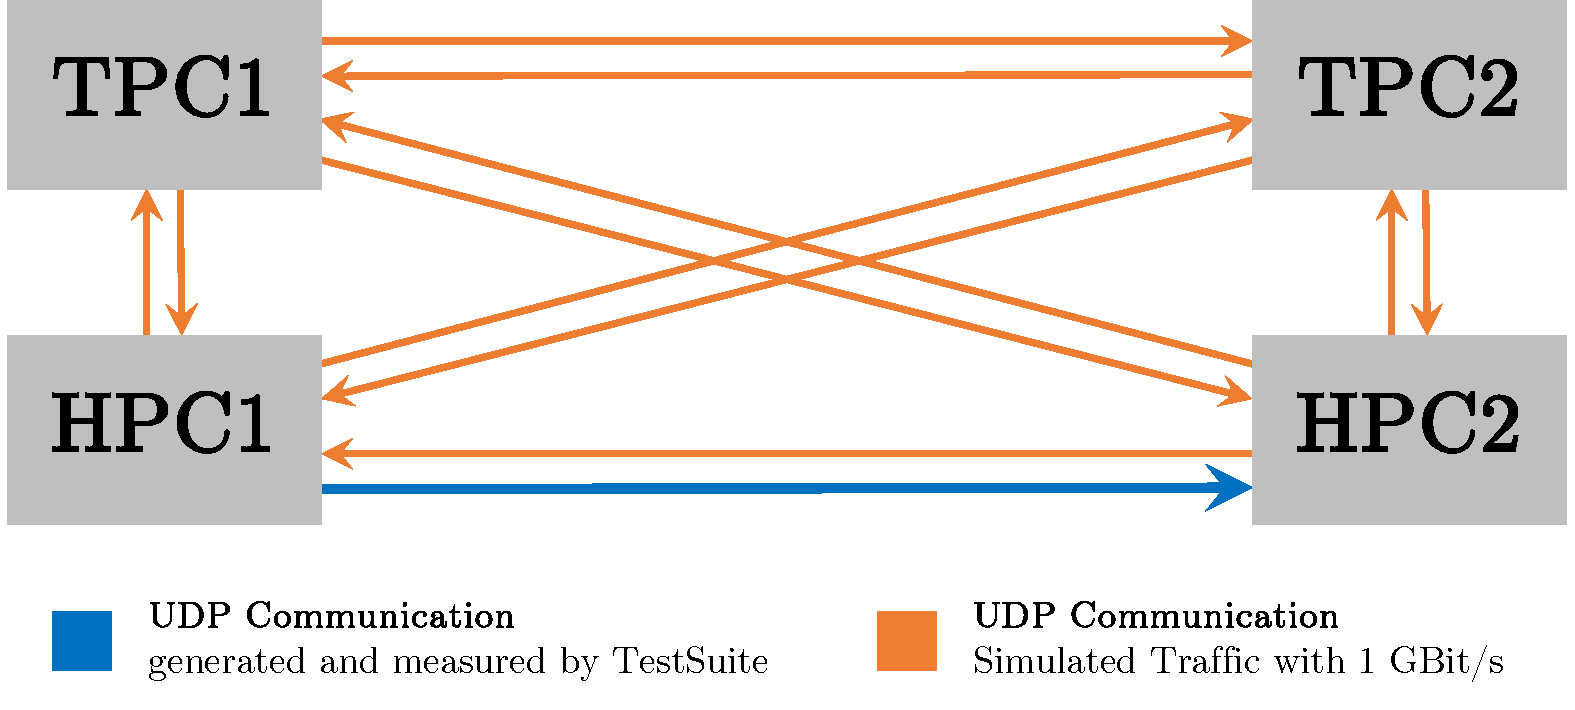
\includegraphics[width=0.8\linewidth]{figures/reliability/star/rel_g_2.pdf}
    \caption{Illustration of the used Systems under Test.}
    \label{fig:realNW}
\end{figure}

Therefore, a realistic load scenario has been developed based on practical experience with a distributed Test Support System, which includes the load on the computer systems as well as on the network. Table \ref{tab:realpc} contains the components of this scenario, which is executed on all computer systems, as well as their analogy in a real distributed Test Support System. These components are generated using stress-ng. Furthermore, the realistic scenario involves UDP network traffic generated with iPerf between all four computer systems of the topology, with a bandwidth limitation of 1 GBit/s per channel, excluding the communication generated and measured by the TestSuite. Figure \ref{fig:realNW} illustrates this, with an example of the High-Performance PCs as the system under test.

This scenario generates a CPU utilization of 56.9\% on a High-Performance PCs without running a test. On a Traffic PCs, the scenario generates a much higher CPU utilization of 100\%, which means the system is fully utilized.

The objective of this campaign is to assess the reliability of the setup under this load. Similar to the previous campaign, datagram sizes of 80 bytes, 8900 bytes, and 65000 bytes will be considered. Additionally, the query function of the TestSuite described in \label{chap:targetcom:query} is used for these tests. A test will be terminated if more than 50 datagram losses occur, as this is considered to be an unreliable communication. The maximum duration of the test is 2 hours.

To examine various bandwidths, the cycle time is systematically increased as well. Starting with an initial value of 0 µs for all datagram sizes, the cycle time is increased in steps of 10 µs. For datagram sizes of 65,000 bytes, the increase starts at a cycle time of 60 µs. This is because, as shown in table \ref{tab:senditertime}, a run through the send loop takes more than 60 µs on average. Testing shorter cycle times would therefore not provide any further insight. The objective of varying the cycle time is to determine the maximum bandwidth possible without experiencing packet loss.

\paragraph{Results}
The campaign was performed with both the High-Performance PCs and the Traffic PCs as the system under test. Although the results differ in absolute terms, they yield the same findings. Therefore, only the results of the High-Performance PCs will be discussed below.

\begin{figure}[h!]
  \centering
  \subcaptionbox{Datagram Size of 8900 Byte\label{fig:resuc3a}}{%
    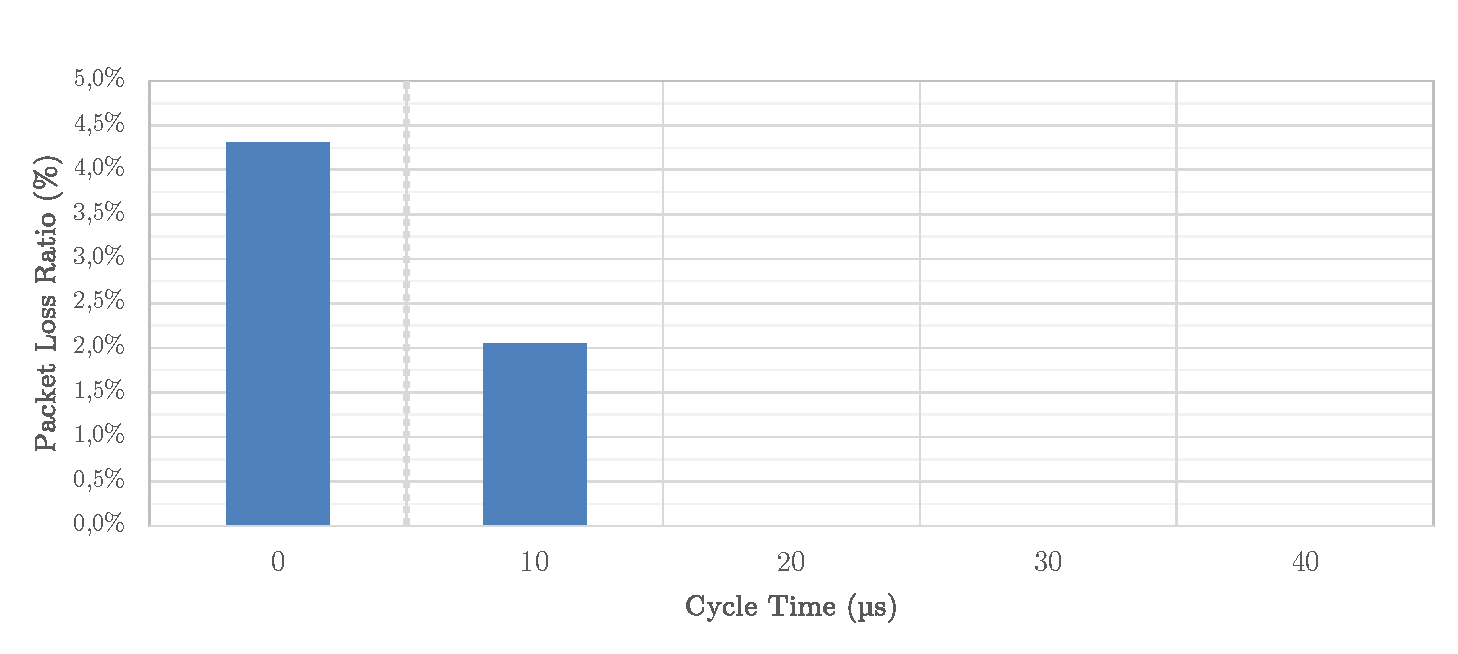
\includegraphics[width=1\textwidth]{figures/reliability/star/rel_d_3a.pdf}
  }
  \subcaptionbox{Datagram Size of 65000 Byte\label{fig:resuc3b}}{%
    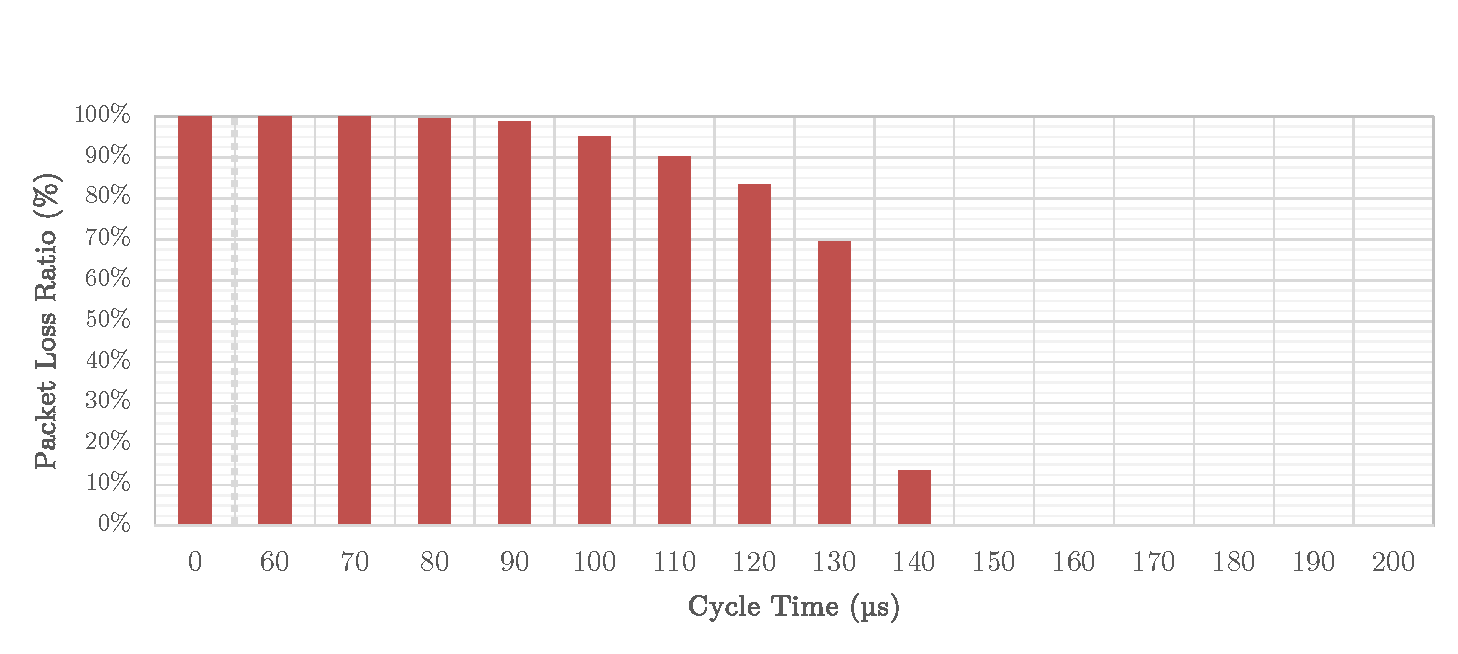
\includegraphics[width=1\textwidth]{figures/reliability/star/rel_d_3b.pdf}
  }
  \caption{Packet Loss Ratio by Cycle Time with High-Performance PCs as System under Test (Campaign „Tests with Realistic Load Scenario“).}
  \label{fig:resuc3}
\end{figure}

Figure \ref{fig:resuc3} displays the percentage of packet losses for various cycle times in tests conducted on High-Performance PCs as a system under test. Results are shown for a datagram size of 8900 bytes in \ref{fig:resuc3a} and 65000 bytes in \ref{fig:resuc3b}. No Loses were detected in tests with a datagram size of 80 bytes.

For a datagram size of 8900 bytes, packet losses were detected at cycle times ranging from 0 µs to 30 µs. Notably, significant packet losses of 4.31\% and 2.05\% occurred at 0 µs and 10 µs, respectively, while only isolated losses were observed at 20 µs and 30 µs. For datagrams with a size of 65000 bytes, significantly higher losses were observed. Over 90\% of packet loss occurred up to a cycle time of 110 µs, after which the percentage of packet loss decreases. No losses occurred starting at a cycle time of 210 µs.

The statistics recorded in the examined computer systems (Standard Interface Statistic and Network Stack Statistic) do not indicate any packet drops, so the sender and receiver can be excluded as the source of the loss.

This turns the switch into a possible source of packet loss. The switch has statistics called 'Tail Drops' that can be viewed for each port in the switch's web interface. These reflect the drops that occur when the output queue of a port is full. The switch will discard data until the output queue is cleared again \cite {reli02}. These described drops occurred during the execution of the tests.

For cycle times of 0 µs and 60 µs with a datagram size of 65000 bytes, the losses can be explained by the possible exceeding of the maximum bandwidth of 10 GBit/s. The average throughput in the tests was 9.0 GBit/s and 8.3 GBit/s, which, in combination with the network load in the realistic scenario (2 GBit/s of incoming traffic on HPC2), operates at the maximum bandwidth with which HPC2 is connected to the switch. However, with a 100 µs cycle time, for example, the average throughput is only 5.2 GBit/s, which means that even in combination with the realistic scenario, the maximum bandwidth is not reached. This also applies to packet losses with a datagram size of 8900 bytes.

At 65000 bytes, exceptionally high losses also occur at cycle times of up to 140 µs, even if the available bandwidth is not exceeded, as explained above with 100 µs as an example. Fragmentation may be one reason for this phenomenon of the high losses, since the entire datagram is discarded when a fragment is lost.

In order to better understand the packet losses, certain tests were repeated and the results of the query requests were recorded. This allows the analysis of the temporal occurrence of packet losses.

\begin{figure}[h!]
    \centering
    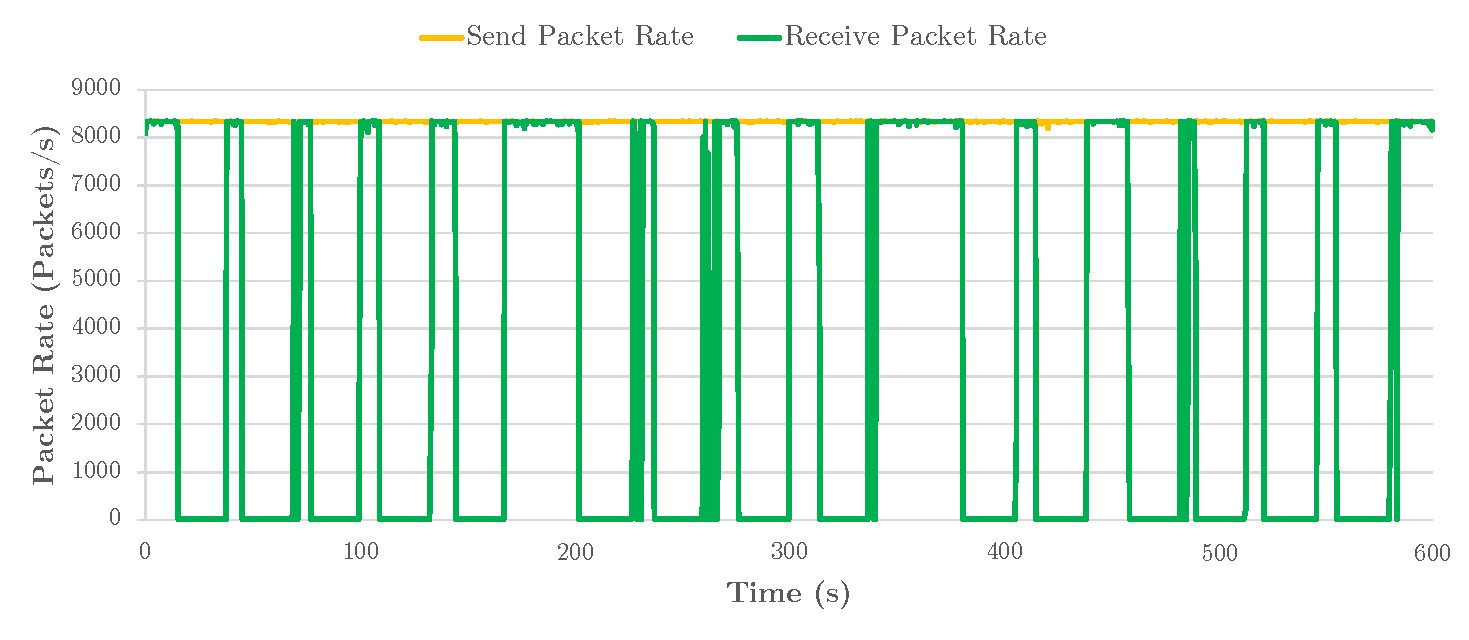
\includegraphics[width=1\linewidth]{figures/reliability/star/rel_d_4.pdf}
    \caption{Sent and Receive Packet Rate over Time for a Test with a Datagram Size of 65000 Byte and a Cycle Time of 120 µs (Campaign „Tests with Realistic Load Scenario“).}
    \label{fig:srpr4}
\end{figure}

Figure \ref{fig:srpr4} displays the send and receive packet rate over time for an example test with a datagram size of 65000 bytes and a cycle time of 120 µs. The average throughput was 4.3 Gbit/s, and there was a 61\% packet loss. The variation in packet losses between this implementation and the results presented in \ref{fig:resuc3} for a cycle time of 120 µs can be attributed to fluctuations.

The diagram shows that the packet losses occur cyclically. It is illustrated that there are phases during which all packets are lost (shown in blue) and phases during which all packets are received (shown in orange). These phases of packet loss have a constant duration of 25 seconds, but the interval between these phases varies.

Based on recorded data, it can be concluded that the packet losses occurred due to an overload the switch. The recorded pattern with the constant loss intervals could indicate an kind of overload protection mechanism of the switch, which prevents the sending of packets. However, the Ethernet switch is a "Black Box", as Cisco does not publish detailed information about the implementation, so the exact cause of the losses cannot be analyzed further. During the tests, all protection mechanisms of this kind, which can be set in the switch interface, were deactivated.

\paragraph{Classification of Results}
This campaign showed that packet losses can occur when the setup is loaded with the realistic scenario. Losses were also observed below the maximum bandwidth. The reason for this is most likely due to switch congestion, which occurs cyclically.

The purpose of the 'Tests with Realistic Load Scenario and Quality of Service' campaign is to investigate the impact of Quality of Service on the results. Meanwhile, the 'Tests with Realistic Load Scenario and custom Network Load Generator' campaign aims to examine the influence of the network load generated by iPerf on the losses.

\subsubsection{Tests with Realistic Load Scenario and Quality of Service}
\paragraph{Motivation and Context}
This test campaign examines the impact of using Quality of Service on the result. The IP header's Differentiated Services field is utilized for this purpose. The TestSuite specifies a priority of 63 for its communication, which is the highest possible value. The switch is also configured to prioritize packets with this priority.

The realistic scenario is executed on all systems involved in the setup, as in the previous campaign. The network traffic generated as part of the scenario is not given preferential treatment by the switch, as no priority is assigned to it.

The test procedure selected for this campaign is the same as the one used for the 'Tests with Realistic Load Scenario' campaign (see \ref{chap:campaignloadscen}). Datagram sizes of 80 bytes, 8900 bytes, and 65000 bytes were taken into consideration. The system under test includes both the High-Performance PCs and the Traffic PCs.

The test campaign examined not only the Intel X710-T2L network interfaces that are the default for the topology, but also the Intel X540-T2, the Inspur X540-T2 and the Lenovo ThinkSystem Marvell QL41134, which were tested with the High-Performance PCs as the system under test.

\paragraph{Results}
In tests with the High-Performance PCs, no packet loss was detected for all datagram sizes tested, with the smallest cycle time tested of 0 µs for 80, 8900, and 65000 bytes. The average throughput achieved in these tests was 91.5 MBit/s for 80 bytes, 7.23 GBit/s for 8900 bytes, and 9.01 GBit/s for 65000 bytes. There were no packet losses in the tests with the alternative network cards (Intel X540-T2, Inspur X540-T2 and Lenovo ThinkSystem Marvell QL41134). The achieved average throughput in these tests is similar to that of the Intel X710-T2L.

Also, no packet loss was detected in the tests with the Traffic PCs with the shortest cycle time. The average throughputs were 52.1 MBit/s for 80 bytes, 4.88 GBit/s for 8900 bytes, and 7.41 GBit/s for 65000 bytes. This also shows that, as mentioned in the first campaign (see \label{chap:relcamp1}), the system load of the traffic PCs has a greater influence on the average throughput achieved by the sender.

However, packet losses were detected in all tests for the traffic generated by iPerf in the context of the realistic load scenario. These effects were caused by the switch, as shown by its statistics.

\paragraph{Classification of Results}
The campaign has demonstrated that reliability can be ensured through the use of quality of service. However, this requires traffic to be prioritized. Nevertheless, packet losses were detected in non-prioritized traffic. Currently, the distributed Test Support System does not provide such prioritization, so no QoS can be applied.

Another finding from this campaign is that the two computer systems in the system under test (client and server) do not cause any packet losses even when under stress from the realistic scenario. This confirms the assumption made in the previous campaign 'Tests with Realistic Load Scenario' based on the recorded statistics.

Furthermore, the campaign has shown that the Intel X540-T2, Inspur X540-T2 and Lenovo ThinkSystem Marvell QL41134 network interfaces have comparable reliability to the Intel X710-T2L.

\subsubsection{Tests with Realistic Load Scenario and Custom Network Load Generator}
\paragraph{Motivation and Context}
The 'Tests with Realistic Load Scenario' campaign (see \ref{chap:campaignloadscen}) has already concluded that the switch suffered from an overload situation. The purpose of this campaign is to further analyze the circumstances that led to packet loss in the switch.

One possible reason for the occurrence of packet losses through the switch is the bursts sent by the network traffic generated by iPerf for the realistic scenario, which cause a short-term overload of the switch. This assumption is supported by the observation that packet losses occur in the switch when executing the realistic scenario in the test setup, even without running a test campaign. Due to the specified bandwidth of 1 GBit/s per channel in the realistic scenario, it is expected that no packet losses will occur as the network's maximum bandwidth is significantly higher.

iPerf utilizes a throttling algorithm to regulate the specified bandwidth. This algorithm monitors the data throughput sent at 100 ms intervals and adjusts it as needed to maintain specified bandwidth \cite{reli03}. Unlike CPU stressors, which run as real-time processes in a realistic load scenario, iPerf is not executed as a real-time process on the system. This can result in iPerf not being allocated sufficient computing time. As a result, the throttling algorithm may make extreme adjustments to achieve the required bandwidth, which may result in data bursts being sent. However, it is not possible to verify this assumption by recording with Wireshark due to hardware limitations.

In this test campaign, a self-programmed network traffic generator based on TestSuite replaces iPerf in the realistic load scenario. Unlike iPerf, this generator does not use a throttling algorithm and therefore does not send any bursts. Furthermore, the process is executed in real-time with a priority of 90, which is higher than that of the stressors but lower than that of TestSuite. The cycle time was configured to ensure a maximum transmission bandwidth of 1 GBit/s.

The test procedure for this campaign was the same as for the 'Tests with Realistic Load Scenario' campaign (see \ref{chap:campaignloadscen}). Datagram sizes of 80 bytes, 8900 bytes, and 65000 bytes were considered. Tests were performed exclusively with the High-Performance PCs as the system under test. Quality of Service was not utilized.

\paragraph{Results}

\begin{figure}[h!]
    \centering
    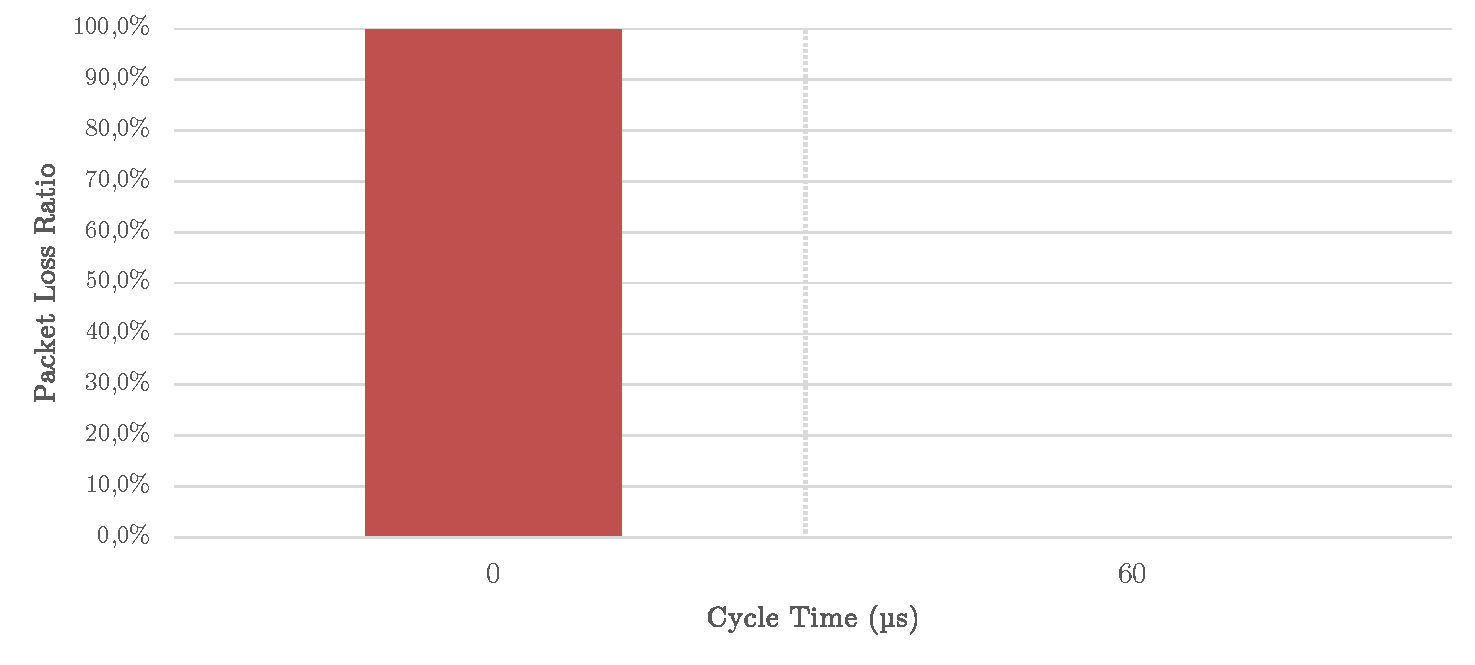
\includegraphics[width=1\linewidth]{figures/reliability/star/rel_d_5.pdf}
    \caption{Packet Loss Ratio by Cycle Time for a Datagram Size of 65000 Byte with High-Performance PCs as System under Test (Campaign „Tests with Realistic Load Scenario and Custom Network Load Generator“).}
    \label{fig:srpr5}
\end{figure}

During the campaign, only packet losses were observed when examining a datagram size of 65000 bytes. At a cycle time of 0 µs, packet losses of 99.9\% were recorded. while no packet losses occurred at a cycle time of 60 µs. These results are illustrated in Figure \ref{fig:srpr5}. It is worth noting that packet drops were again only reported by the switch.

A major reason for the high number of packet losses at 65000 byte datagram size and 0 µs cycle time is the fact that the maximum bandwidth of 10 Gbps is exceeded, as the average throughput in the test is 9.1 Gbps. Additionally, packet loss is increased by the use of fragmentation.

\paragraph{Classification of Results}
Compared to using iPerf (see \ref{chap:campaignloadscen}), a separate network stressor significantly reduces packet losses. This suggests that iPerf generates bursts that overload the switch and cause packet loss. However, it should be noted that the systems in the distributed test support system are asynchronous, meaning they can also send out bursts that should not overload the network.

\subsection{Insights}
The investigation of the star topology with a switch in the center has revealed that an Ethernet switch is unsuitable for use in the distributed Test Support System. The switch was found to be the cause of packet loss, particularly in connection with burst traffic.

Another concern is that the maximum bandwidth at which each participant is connected to the switch may be exceeded. Since the distributed Test Support System operates as an asynchronous system, such an exceedance cannot be excluded.

Regarding the computer systems, the investigation showed that a memory load that provokes a constant memory overflow can lead to packet loss. However, it was also found that both High-Performance PC and Traffic PC systems do not experience packet losses when subjected to a load similar to that in a real Test Support System.

Furthermore, in addition to the standard network interfaces in the topology, the Intel X540-T2, Inspur X540-T2, and Lenovo ThinkSystem Marvell QL41134 network interfaces were also examined, and no reduction in reliability based on packet loss was found, making them equally suitable for use in a distributed Test Support System.




\section{Reliability Analysis of the Star Topology with the iHawk in the Centre}

\subsection{System under Test}
The key takeaway from the previous reliability tests (see 3.2.3) is that the use of an Ethernet switch in the distributed AIDASS is unsuitable, as it leads to a significant number of lost packets. The behavior of the switch was also found to be unreliable and sometimes unpredictable.












